% !TeX root = main.tex
% SIGma Fall 2026. Shared theme from the two preceding presentations.
\documentclass[aspectratio=169]{beamer}
\usepackage{../sty/slides}
\usepackage{../sty/sigma/sigma}
\usepackage{../sty/math}
\usepackage{../sty/stat}
\usepackage{../sty/algo}
\usepackage{../sty/code}
\usepackage{tikz}
\usetikzlibrary{arrows.meta,positioning}
\title{Complexity and Linear Programming}
\subtitle{9/14/26}
\author{Mihir Tandon}
\begin{document}
\begin{frame}\titlepage\end{frame}

\section{Big O Notation}
\begin{frame}[fragile]{How many computations does this do?}
\begin{pycode}
Algorithm Sum(A, n):
    total = 0
    for i = 1 to n
        total = total + A[i]
    return total
\end{pycode}
\begin{itemize}
\item How many additions does this algorithm perform on an array of $n$ values?
\pause
\item \textbf{Answer:} Exactly $n$ additions. Doubling the input doubles this count.
\end{itemize}
\end{frame}

\begin{frame}[fragile]{What changes with two loops?}
\begin{pycode}
Algorithm ComparePairs(A, n):
    for i = 1 to n
        for j = i + 1 to n
            compare(A[i], A[j])
\end{pycode}
\begin{itemize}
\item How many comparisons does this algorithm perform?
\pause
\item \textbf{Answer:} $(n-1)+(n-2)+\cdots+1=\frac{n(n-1)}{2}$ comparisons.
\pause
\item For large $n$, doubling the input roughly quadruples this count.
\end{itemize}
\end{frame}

\begin{frame}[fragile]{What if the input keeps shrinking?}
\begin{pycode}
Algorithm Halve(n):
    while n > 1
        n = floor(n / 2)
\end{pycode}
\begin{itemize}
\item For an integer $n\geq1$, how many times does the loop divide by two?
\pause
\item \textbf{Answer:} $\lfloor\log_2 n\rfloor$ times. For $n=16$, the values are $16,8,4,2,1$, so there are four divisions.
\pause
\item Let $T(n)$ count the number of operations. Big O describes how that count grows with the input size.
\end{itemize}
\end{frame}

\begin{frame}{Big O notation}
\begin{itemize}
\item We write $T(n)=O(g(n))$ if constants $c>0$ and $n_0$ exist such that
\[0\leq T(n)\leq c\,g(n)\qquad\text{for all }n\geq n_0.\]
\pause
\item The constant $c$ allows a fixed multiplicative difference. The threshold $n_0$ lets us ignore small inputs.
\pause
\item For example, $3n+7\leq4n$ whenever $n\geq7$. Therefore, $3n+7=O(n)$.
\pause
\item Big O gives an upper bound. A linear runtime is also $O(n^2)$, although that bound is less useful.
\end{itemize}
\end{frame}

\begin{frame}[fragile]{A convex hull recurrence}
\begin{itemize}
\item Consider a divide-and-conquer convex hull algorithm on $n$ points sorted by $x$-coordinate.
\end{itemize}
\pause
\begin{pycode}
Hull(P):
    if |P| <= 3: return the hull of P
    split P into left and right halves
    H_left  = Hull(left)
    H_right = Hull(right)
    return MergeHulls(H_left, H_right)
\end{pycode}
\pause
\begin{itemize}[<+->]
\item The recursive calls solve two subproblems of size $n/2$. The merge finds the upper and lower tangents in $O(n)$ time.
\item This gives the recurrence $T(n)=2T(n/2)+O(n)$.
\item The recursion has $O(\log n)$ levels, and each level performs $O(n)$ total merge work.
\item Therefore $T(n)=O(n\log n)$.
\end{itemize}
\end{frame}

\begin{frame}{Why growth rates matter}
\centering
\begin{tabular}{lrr}
Growth function & $n=10$ & $n=100$\\\hline
$n$ & 10 & 100\\
$n\log_2 n$ & $\approx33$ & $\approx664$\\
$n^2$ & 100 & 10,000\\
$n^3$ & 1,000 & 1,000,000\\
$2^n$ & 1,024 & $\approx1.27\times10^{30}$
\end{tabular}
\vspace{0.4cm}
\end{frame}

\section{Linear Programming}
\frame{\sectionpage}
\begin{frame}{Linear programming}
\begin{itemize}
\item A \textbf{linear program (LP)} optimizes a linear objective subject to linear inequalities.
\pause
\[
\begin{aligned}
\min\quad &c_1x_1+\cdots+c_dx_d\\
\text{subject to}\quad &a_{i1}x_1+\cdots+a_{id}x_d\leq b_i
\quad (i=1,\ldots,n),\\
&x_1,\ldots,x_d\in\mathbb R.
\end{aligned}
\]
\pause
\item The vector $c=(c_1,\ldots,c_d)$ is the \textbf{objective vector}. It assigns a cost to each variable, and $c^Tx$ is the total cost we minimize.
\pause
\item Each row vector $a_i=(a_{i1},\ldots,a_{id})$ gives an inequality $a_i^Tx\leq b_i$, which defines a \textbf{halfspace}. Their intersection is the feasible region.
\pause
\item We can also maximize. Here, programming means mathematical optimization.
\end{itemize}
\end{frame}

\begin{frame}{A production problem}
\begin{itemize}
\item A workshop makes tables and chairs. It has 7 planks of wood and enough time to assemble 5 items.
\pause
\end{itemize}
\begin{center}
\begin{tabular}{lcc}
 & Table & Chair\\\hline
Wood required & 2 planks & 1 plank\\
Profit & 3 dollars & 2 dollars
\end{tabular}
\end{center}
\pause
\begin{itemize}
\item Let $x$ count tables and $y$ count chairs. Ignoring whole-number restrictions for now, the LP is
\[
\begin{aligned}
\max\quad &3x+2y\\
\text{subject to}\quad &2x+y\leq7,\qquad x+y\leq5,\\
&x,y\in\mathbb R_{\geq0}.
\end{aligned}
\]
\end{itemize}
\end{frame}

\begin{frame}{The geometry of the production LP}
\begin{columns}
\begin{column}{0.45\textwidth}
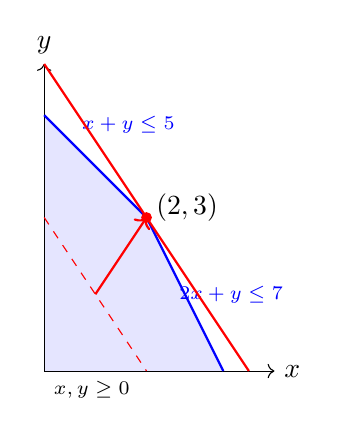
\begin{tikzpicture}[scale=0.65]
\fill[blue!10] (0,0)--(3.5,0)--(2,3)--(0,5)--cycle;
\draw[->] (0,0)--(4.5,0) node[right] {$x$};
\draw[->] (0,0)--(0,6) node[above] {$y$};
\draw[blue,thick] (0,5)--(2,3)--(3.5,0);
\node[blue, font=\scriptsize, above right] at (0.55,4.45) {$x+y\leq5$};
\node[blue, font=\scriptsize, below right] at (2.45,1.85) {$2x+y\leq7$};
\node[font=\scriptsize, below right] at (0,0) {$x,y\geq0$};
\draw[red,dashed] (0,3)--(2,0);
\draw[red,thick] (0,6)--(4,0);
\draw[->,red,thick] (1,1.5)--(2,3);
\fill[red] (2,3) circle (3pt);
\node[right] at (2,3.2) {$(2,3)$};
\end{tikzpicture}
\end{column}
\begin{column}{0.53\textwidth}
\begin{itemize}
\item Each inequality defines a half-plane in two dimensions, or a halfspace in $d$ dimensions. Their intersection is the \textbf{feasible region}.
\pause
\item Here, $x,y\geq0$, $2x+y\leq7$, and $x+y\leq5$ define the shaded region.
\pause
\item To maximize $3x+2y$, move the line $3x+2y=t$ toward larger $t$. The last contact occurs at $(2,3)$, with value $12$.
\end{itemize}
\end{column}
\end{columns}
\end{frame}

\begin{frame}{Seidel's LP algorithm}
\begin{itemize}[<+->]
\item Let $H=\{h_1,\ldots,h_n\}$ be halfspace constraints in $\mathbb R^d$, and let $c$ be an objective vector. We maximize $c^Tx$ over their intersection.
\item Seidel adds the constraints in random order while maintaining the optimum for those seen so far.
\end{itemize}
\end{frame}

\begin{frame}[fragile]{Seidel pseudocode}
\begin{pycode}
SeidelLP(H, c, d):
    randomly order the constraints in H
    x = solve a constant size base case
    for i = 1 to number of constraints:
        if x violates constraint h_i:
            B = boundary of h_i
            x = SeidelLP(earlier constraints on B, c, d-1)
    return x
\end{pycode}
\pause
\begin{itemize}
\item The recursive call only uses earlier constraints and searches on the boundary of the violated constraint.
\end{itemize}
\end{frame}

\begin{frame}{A two-dimensional linear program}
\centering
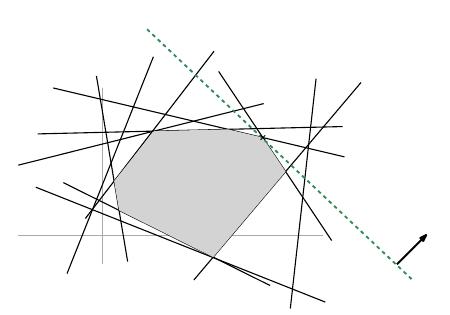
\includegraphics[width=0.72\textwidth,height=0.76\textheight,keepaspectratio]{images/seidel_lp_overview.png}
\blfootnote{Figure adapted from 15-451/651 Lecture 14, October 21, 2015.}
\end{frame}

\begin{frame}{Seidel Example: adding one constraint}
\begin{itemize}[<+->]
\item Suppose we know the optimum for the first $m-1$ constraints, then add $a_m^Tx\leq b_m$.
\item If the old optimum satisfies it, nothing changes.
\item Otherwise, the new optimum lies on the boundary $a_m^Tx=b_m$. Restricting to this boundary reduces the problem from $d$ dimensions to $d-1$.
\end{itemize}
\end{frame}

\begin{frame}{Adding one constraint}
\centering
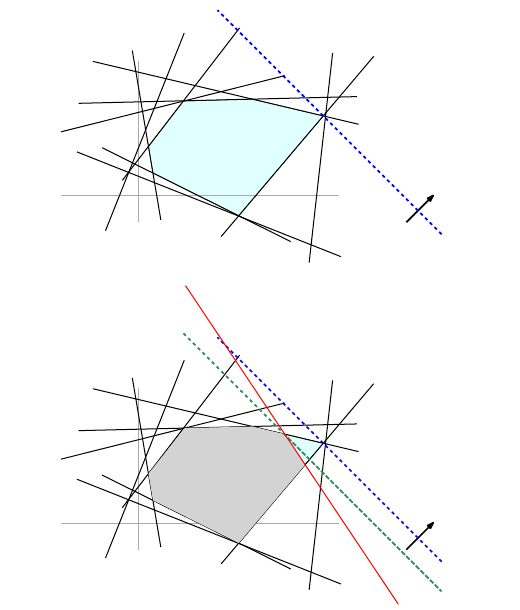
\includegraphics[width=0.62\textwidth,height=0.76\textheight,keepaspectratio]{images/seidel_lp_insert.png}
\blfootnote{Figure adapted from 15-451/651 Lecture 14, October 21, 2015.}
\end{frame}

\begin{frame}{Seidel's expected-time recurrence}
\begin{itemize}[<+->]
\item Let $T(d,n)$ be the expected time for $n$ constraints in dimension $d$. At step $i$, the algorithm first tests the new constraint in $O(d)$ time.
\item At the best point, at most $d$ constraints are needed to fix its position. Because the order is random, constraint $i$ has probability at most $d/i$ of changing that point and starting a recursive call.
\item A recursive call solves an LP with $i-1$ earlier constraints in dimension $d-1$:
\[
T(d,i)\leq T(d,i-1)+O(d)+\frac{d}{i}T(d-1,i-1).
\]
\end{itemize}
\end{frame}

\begin{frame}{Deriving $O(d!\,n)$}
\begin{itemize}[<+->]
\item Sum the one-step recurrence over $i=1,\ldots,n$:
\[
T(d,n)\leq\sum_{i=1}^n\left(O(d)+\frac{d}{i}T(d-1,i-1)\right).
\]
\item Induct on $d$. Assume $T(d-1,i-1)\leq K(d-1)!(i-1)$ for every $i$.
\[
\frac{d}{i}T(d-1,i-1)
\leq\frac{d}{i}K(d-1)!(i-1)
\leq Kd!.
\]  
\item Every one of the $n$ steps therefore has expected cost $O(d!)$. Thus $T(d,n)=O(d!\,n)$. The base case $d=1$ is a linear scan.
\end{itemize}
\end{frame}

\begin{frame}{Why fixed-dimensional LP is useful}
\begin{itemize}[<+->]
\item In a fixed dimension $d$, Seidel's randomized incremental algorithm takes expected $O(d!\,n)$ time. 
\pause
\item The method is practical when the dimension stays small.
\end{itemize}
\end{frame}

\section{Integer Linear Programming}
\frame{\sectionpage}
\begin{frame}{From LP to integer linear programming}
\begin{itemize}
\item An \textbf{Integer Linear Program (ILP)} adds integer restrictions to an LP. Counts must be whole numbers, and yes-or-no decisions use $0$ or $1$.
\pause
\[
\begin{array}{ll}
\text{LP:} & \min c^Tx\quad\text{subject to }Ax\leq b,\quad x\in\mathbb R^d,\\[0.25cm]
\text{ILP:} & \min c^Tx\quad\text{subject to }Ax\leq b,\quad x\in\mathbb Z^d.
\end{array}
\]
\pause
\item The inequalities still define the same region. The ILP only allows its integer points.
\pause
\item LP has polynomial-time algorithms, but general ILP is NP-hard.
\end{itemize}
\end{frame}
\begin{frame}{An ILP example}
\begin{itemize}[<+->]
\item A workshop makes tables ($x$) and chairs ($y$). It has four units of each of two resources. A table uses $(2,1)$ units and a chair uses $(1,2)$ units.
\item The integer linear program is
\[
\begin{aligned}
\max\quad &3x+2y\\
\text{subject to}\quad &2x+y\leq4,\\
&x+2y\leq4,\\
&x,y\in\mathbb Z_{\geq0}.
\end{aligned}
\]
\item The LP \textit{relaxation} (ignoring integer constraints) has $x=y=\frac43$ and value $\frac{20}{3}$. The ILP optimum is $(x,y)=(2,0)$ with value $6$.
\end{itemize}
\end{frame}

\begin{frame}{How branch and bound works}
\begin{itemize}[<+->]
\item First ignore the integer restrictions and solve the LP relaxation. Its objective value bounds every integer solution in that branch.
\item If the LP solution is fractional, choose one fractional variable and split the search into two cases, such as $x\leq\lfloor x^*\rfloor$ and $x\geq\lceil x^*\rceil$.
\item Whenever the solver finds a valid integer solution, it stores its value as the incumbent.
\item Prune a branch when it is infeasible, already integer, or its LP bound cannot improve the incumbent.
\item Once every branch is solved or pruned, the incumbent is an optimal ILP solution.
\end{itemize}
\end{frame}

\begin{frame}{Branch and bound: search and prune}
\begin{itemize}[<+->]\small
\item The LP relaxation has upper bound $\frac{20}{3}$ and fractional value $x=\frac43$.
\item Branch into $x\leq1$ and $x\geq2$.
\item The $x\geq2$ branch gives $(2,0)$ with value $6$. It becomes the incumbent.
\item The $x\leq1$ branch has LP upper bound $6$, so it cannot improve the incumbent and is pruned.
\end{itemize}
\centering
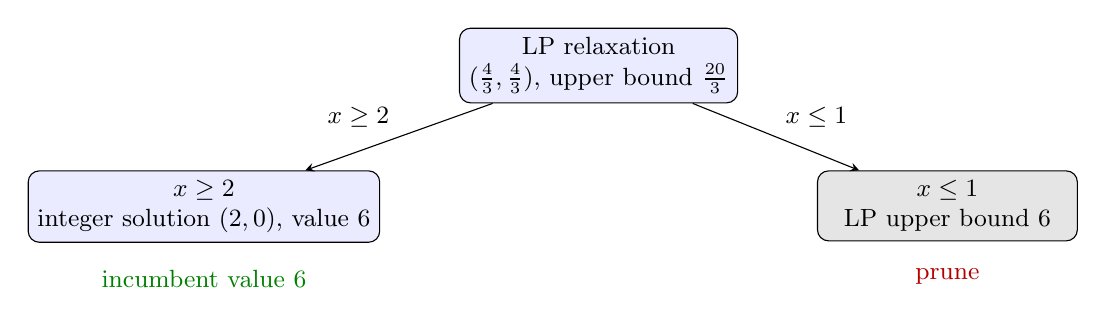
\begin{tikzpicture}[>=stealth, every node/.style={font=\small, align=center},
  box/.style={draw, rounded corners, fill=blue!8, minimum width=3.3cm, minimum height=0.7cm},
  prune/.style={draw, rounded corners, fill=gray!20, minimum width=3.3cm, minimum height=0.7cm}]
  \node[box] (root) {LP relaxation\\$(\frac43,\frac43)$, upper bound $\frac{20}{3}$};
  \node[box, below left=0.85cm and 1.0cm of root] (left) {$x\geq2$\\integer solution $(2,0)$, value $6$};
  \node[prune, below right=0.85cm and 1.0cm of root] (right) {$x\leq1$\\LP upper bound $6$};
  \draw[->] (root) -- node[above left] {$x\geq2$} (left);
  \draw[->] (root) -- node[above right] {$x\leq1$} (right);
  \node[below=0.22cm of left, text=green!50!black] {incumbent value $6$};
  \node[below=0.22cm of right, text=red!70!black] {prune};
\end{tikzpicture}
\end{frame}

\begin{frame}{ILP solvers in Python}
\begin{itemize}[<+->]
\item In python, we just have to describe variables, linear constraints, and an objective. A solver performs the search.
\item \texttt{scipy.optimize.milp} provides a direct interface to the HiGHS mixed-integer solver. Modeling tools such as PuLP and Pyomo can target several solvers.
\item General ILP solvers combine presolve, LP relaxations, cutting planes, heuristics, and branch-and-bound.
\item When the solver reports optimal status, it has proved that no better feasible integer solution exists, subject to numerical tolerances.
\end{itemize}
\end{frame}



\begin{frame}{Questions?}
\end{frame}

\end{document}
